\begin{figure*}[t]
    \renewcommand{\arraystretch}{1.5}
    \begin{subfigure}[t]{0.6\textwidth}
        \raisebox{2.1cm}{
        
        \begin{tabular}{ l||m{2.8cm}|m{2.5cm}  }
            \centering
            Task & VAL (Ours) \; \; \; \; Offline $\rightarrow$ Online & CCRIG  \; \; \; \; \; \; Offline $\rightarrow$ Online \\
            \hline
            (1) Pickup shoe & $12.5\%$ $\rightarrow$ $\textbf{50\%}$ & $0\%$ $\rightarrow$ $16.6\%$ \\
            (2) Drawer closing & $25\%$ $\rightarrow$ $\textbf{100\%}$ & $0\%$ $\rightarrow$ $12.5\%$ \\
            (3) Drawer opening & $62.5\%$ $\rightarrow$ $\textbf{100\%}$ & $0\%$ $\rightarrow$ $0\%$ \\
            (4) Place object in tray & $25\%$ $\rightarrow$ $\textbf{75\%}$ & $0\%$ $\rightarrow$ $0\%$ \\
            (5) Lid on pot & $37.5\%$ $\rightarrow$ $\textbf{87.5\%}$ & $0\%$ $\rightarrow$ $0\%$ \\
        \end{tabular}
        }
    \end{subfigure}
    \begin{subfigure}[t]{0.05\textwidth}
        \vspace{-3.3cm}
        (1)
        \vspace{0.3cm}
        
        (2)
        \vspace{0.3cm}
        
        (3)
        \vspace{0.3cm}
        
        (4)
        \vspace{0.3cm}
        
        (5)
    \end{subfigure}
    \begin{subfigure}[t]{0.34\textwidth}
        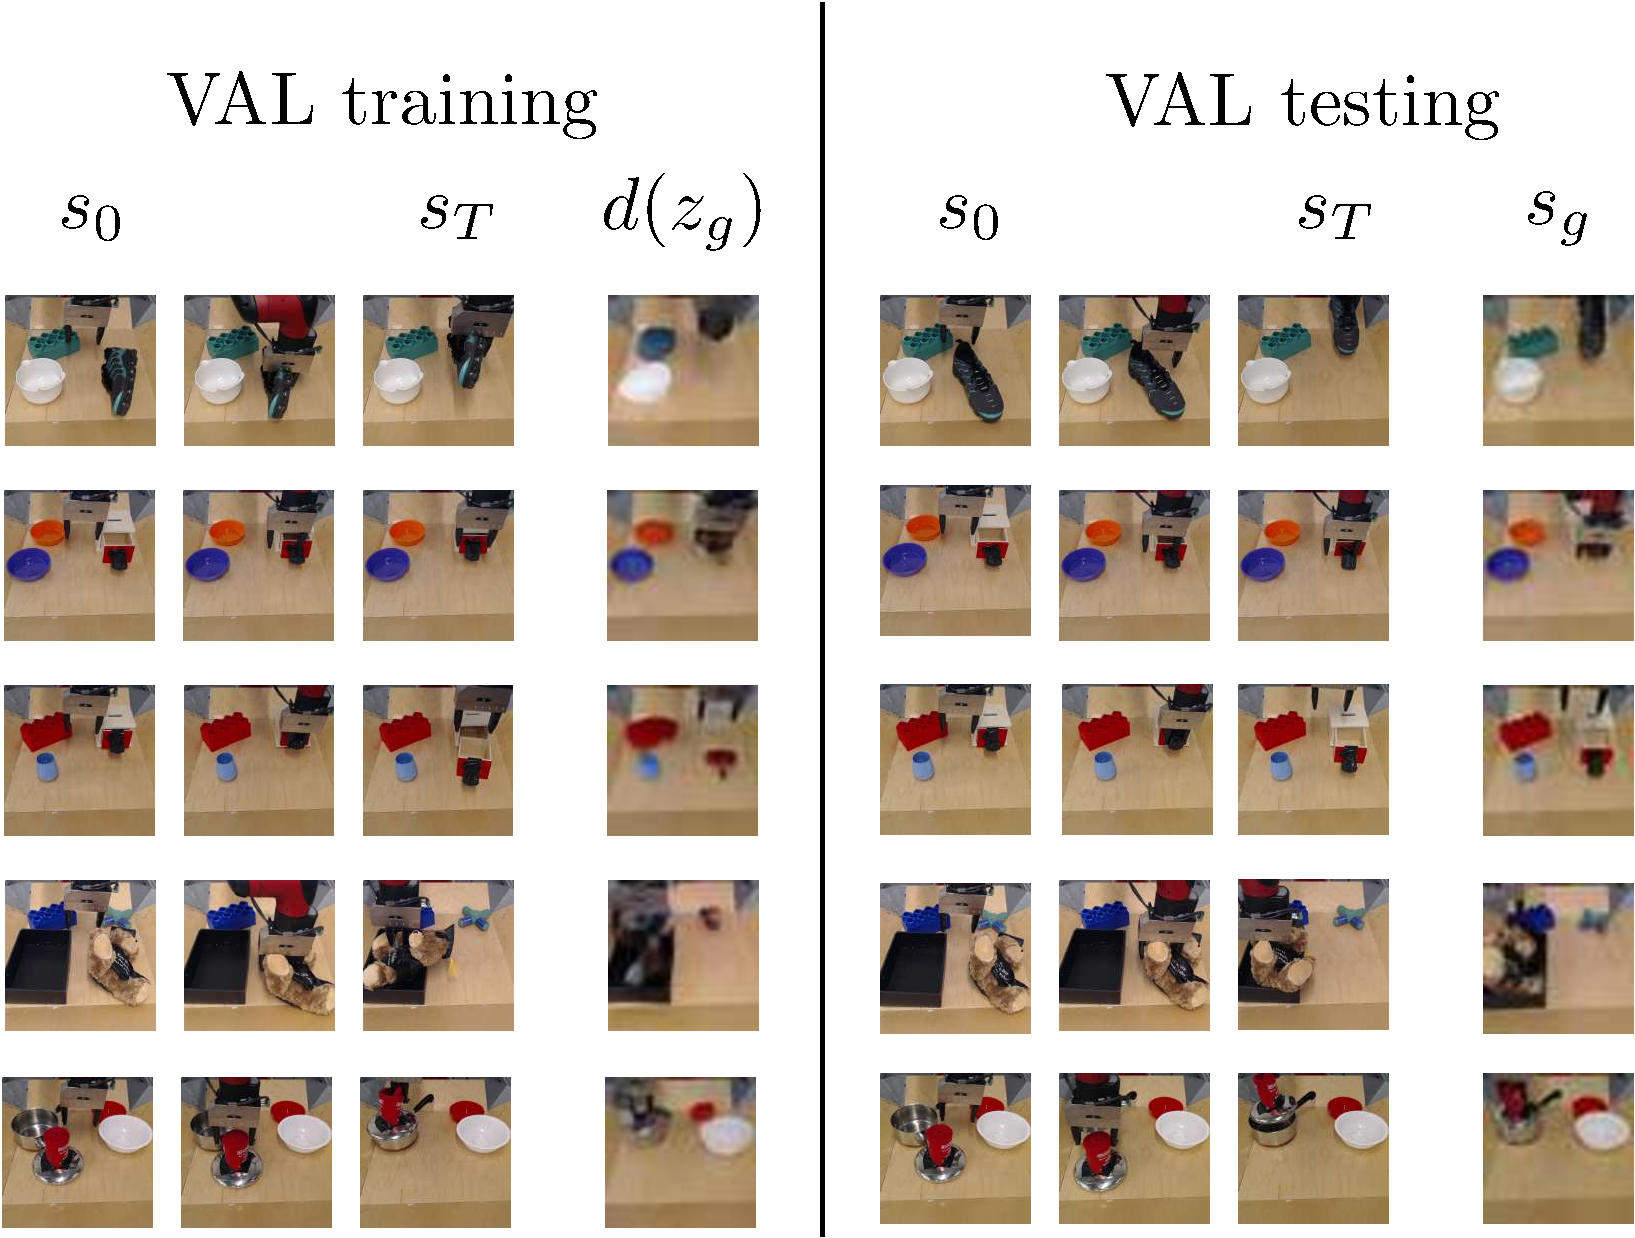
\includegraphics[width=0.99\textwidth]{val/imgs/fig_rollouts_v3.pdf}
    \end{subfigure}
    
    \caption{Real-world results. Left, success rates per method for the five tasks tested. We report the offline performance, followed by the performance after five minutes of online fine-tuning. With VAL, we see reasonable initial offline performance followed by significant improvement on all tasks. Meanwhile CCRIG fails to succeed any of the tasks. Right, film strips of VAL during training (left, with decoded affordance proposals) and testing (right, with goal images) are visualized. Videos are available at \url{https://sites.google.com/view/val-rl}}
    \label{fig:real-world-results}
    % \vspace{-0.5cm}
\end{figure*}